
\documentclass[final,hyperref={pdfpagelabels=false}]{beamer}

\usepackage{grffile}
\usepackage{graphics}
\usepackage{color}
\usepackage[english]{babel}
\usepackage[orientation=portrait,size=a0,scale=1.4,debug]{beamerposter}
\usepackage{array,booktabs,tabularx}
\usepackage{subfigure}
\usepackage[T1]{fontenc}

\usepackage{lmodern} % Use Latin Modern instead of Computer Modern


\newcommand*{\myfont}{\fontfamily{ptm}\selectfont}
\DeclareTextFontCommand{\textmyfont}{\myfont}

% \usepackage[sfdefault]{roboto}  %% Option 'sfdefault' only if the base font of the document is to be sans serif

         
\mode<presentation> 
{  %% check http://www-i6.informatik.rwth-aachen.de/~dreuw/latexbeamerposter.php for examples
  \usetheme{_bscholl_2018}    %% you should define your own theme e.g. for big headlines using your own logos 
}

\definecolor{Blue}{rgb}{0,0,1}
\definecolor{Orange}{rgb}{1,0.5,0}
\boldmath

\newcolumntype{Z}{>{\centering\arraybackslash}X} % centered tabularx columns

\newcommand{\pphantom}{\textcolor{white}} % phantom introduces a vertical space in p formatted table columns??!!


\newlength{\columnheight}

\setlength{\columnheight}{105cm}

% Corrects a beamer bug:
%
\providecommand\thispdfpagelabel[1]{}

\listfiles

%%%%%%%%%%%%%%%%%%%%%%%%%%%%%%%%%%%%%%%%%%%%%%%%%%%%%%%%%%%%%%%%%%%%%%%%%%%%%%%%%%%%%%

\graphicspath{{figures/}}
 
\title{\huge\textbf{A Study on Gradient Boosting Classifiers}\\$\phantom{a}$\bigskip\bigskip
}    



\author{\textbf{Juliano Garcia de Oliveira}\\Advisor: Prof. Dr. Roberto Hirata Jr.\\$\phantom{a}$\bigskip\bigskip}



\institute[IME-USP]{\large{Department of Computer Science -- Institute of Mathematics and Statistics \\ University of São Paulo}}

\date[December, 2019]{December 3, 2019}

%%%%%%%%%%%%%%%%%%%%%%%%%%%%%%%%%%%%%%%%%%%%%%%%%%%%%%%%%%%%%%%%%%%%%%%%%%%%%%%%%%%%%%

\begin{document}
\begin{frame}

\begin{columns}

\begin{column}{.497\textwidth}
\begin{beamercolorbox}[center,wd=\textwidth]{postercolumn}
        
\begin{minipage}[T]{.95\textwidth}  % tweaks the width, makes a new \textwidth
                     
\parbox[t][\columnheight]{\textwidth}
{ 
% must be some better way to set the the height, width and textwidth simultaneously
% Since all columns are the same length, it is all nice and tidy.  You have to get the height empirically
% ---------------------------------------------------------%
% fill each column with content  
                    
\begin{block}{Introduction}
\parbox[t][]{0.95\textwidth}  % parbox allows full justification
{     
\begin{myfont}
    

    Trypanosomatida is a family of pathogenic protozoa, whose one of most prominent members is {\em Trypanosoma brucei}, the parasite behind the African sleeping sickness. Given the public health significance of this protozoan, its biology is int
    , in a parallelized fashion, on several specific DNA locations called replication origins. \textmyfont{There are three types of origins: constitutive, flexible and dormant; the latter is only initiated as a response to DNA replication failure}. Recently, putative constitutive origins were mapped for {\em T. brucei} through MFA-seq assays [1]. Moreover, a DNA replication dynamic model was implemented in a Python-based simulator called ReDyMo [2]. Simulations of this model highlighted the relevance of replication-transcription conflicts on the origin firing distribution along the genome [2]. However, whether this parasite has or not dormant origins remained as open question.
\end{myfont}
}
\end{block}


\begin{block}{\protect Gradient Boosting Machines}
\parbox[t][]{0.95\textwidth}
{
\begin{itemize}
    \item {\bf General objective:} to computationally test the hypothesis of the presence of dormant origins in {\em T. brucei} strain TREU927.
    \begin{enumerate}
        \item it will require the designing of a multiscale model
        \item this model will be used to simulate the dynamics of a parasite population in exponential growth
    \end{enumerate}
    \bigskip
    \item {\bf Specific goal:} to port the ReDyMo simulator to C++ in order to:
\end{itemize}
}
\end{block}


\begin{block}{\protect Study Methodology}
\parbox[t][]{0.95\textwidth}
{
\begin{figure}
    \centering
    \scalebox{0.2}{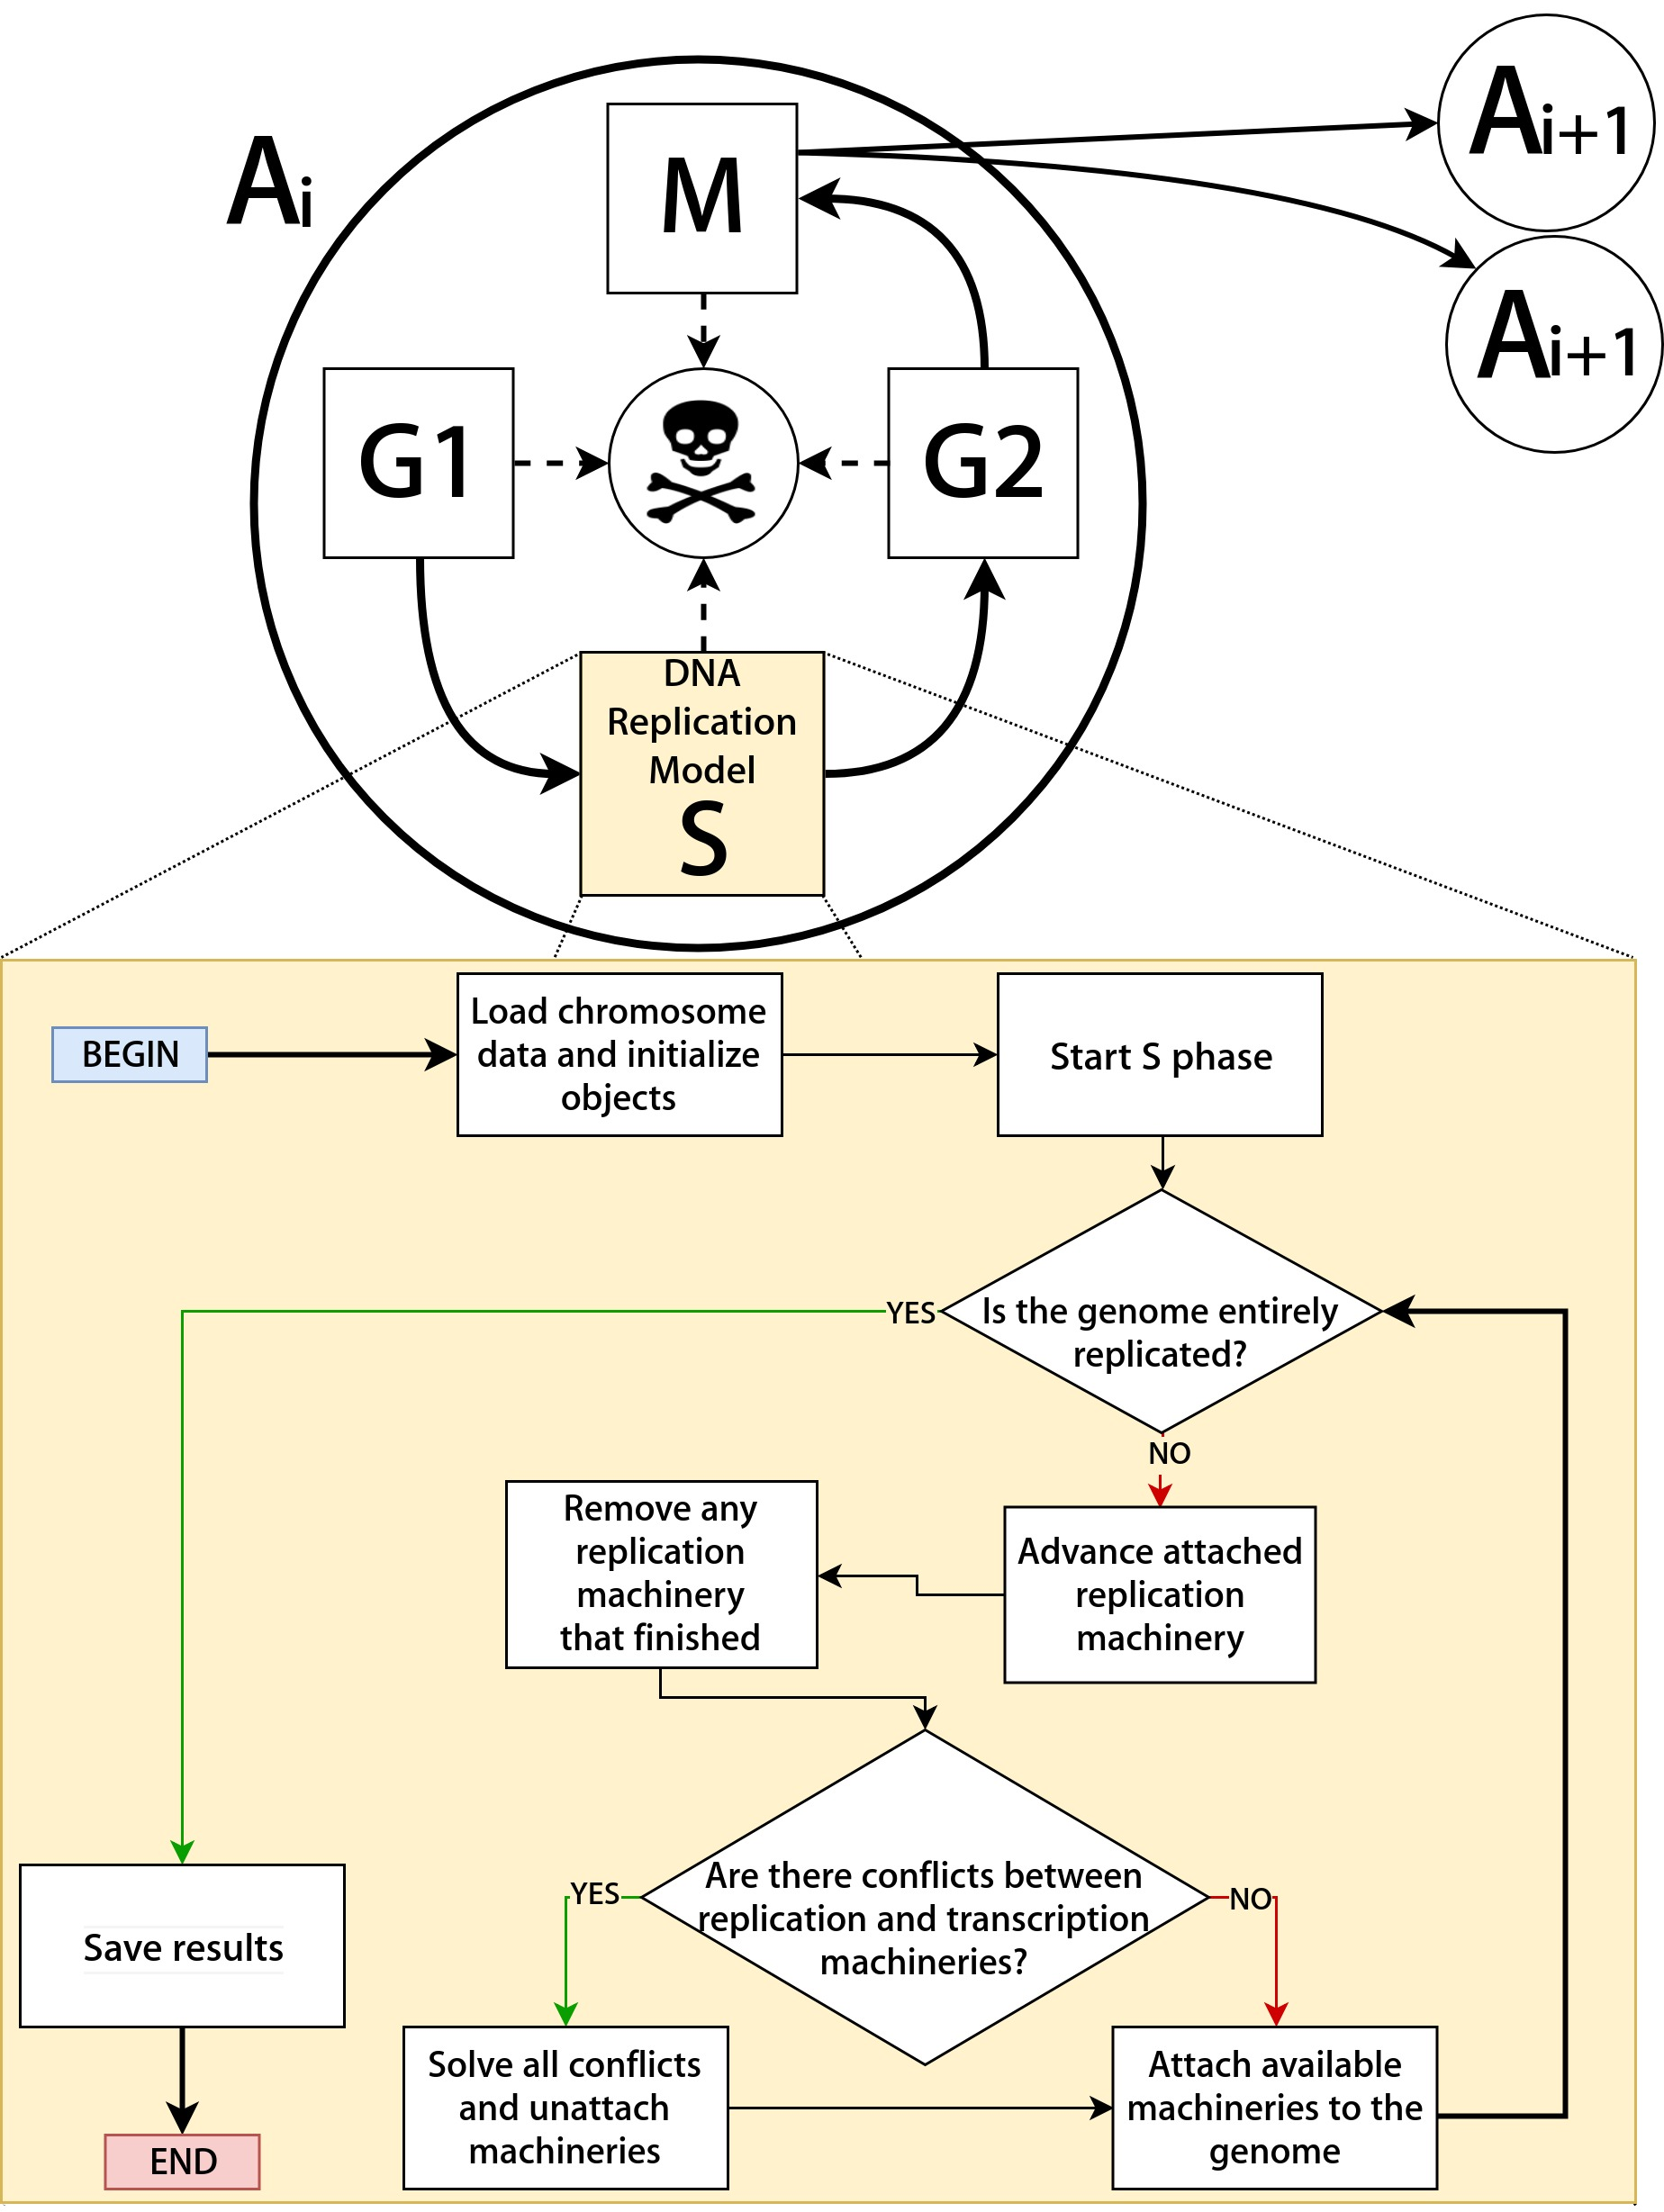
\includegraphics[trim = 0mm 0mm 0mm 0mm, clip=true]{Model_Layers.jpg}}
    \label{fig:model}
\end{figure}
{\bf Fig.~1: Diagram of the proposed agent-based multiscale model.} Each cell (agent) has an outer and an inner layers. In the outer layer it is simulated all phases of cell cycle (G1, S, G2/M). Each cell either finishes its cycle successfully (so it spawns two daughter cells) or dies (and is removed from simulation). The S-phase duration and success is given by the DNA replication dynamic model contained in the inner layer (orange box). 
}
\end{block}

      \begin{block}{References}
	\scriptsize
      \smallskip
        [1] Tiengwe et al. Cell Reports (2012). DOI: \href{https://doi.org/10.1016/j.celrep.2012.06.007}{10.1016/j.celrep.2012.06.007}\\
        \bigskip
        [2] da Silva et al. Submitted (2018). DOI: \href{https://doi.org/10.1101/398016 }{10.1101/398016 }\\
\end{block}

\vfill  % last vfill is important to avoid page duplication!

} % end \parbox
                        
\end{minipage}
\end{beamercolorbox}
\end{column}
% ---------------------------------------------------------%
% end the column

% ---------------------------------------------------------%
% Set up a column 
\begin{column}{.497\textwidth}
\begin{beamercolorbox}[center,wd=\textwidth]{postercolumn}
\begin{minipage}[T]{.95\textwidth} % tweaks the width, makes a new \textwidth         
          
\parbox[t][\columnheight]{\textwidth}
{ 
% must be some better way to set the the height, width and textwidth simultaneously
% Since all columns are the same length, it is all nice and tidy.  You have to get the height empirically
% ---------------------------------------------------------%
% fill each column with content  
                     

\begin{block}{\protect Statistical Analysis}
\parbox[t][]{0.95\textwidth}
{
\begin{figure}
    \centering
    \scalebox{1.2}{
        \centerline{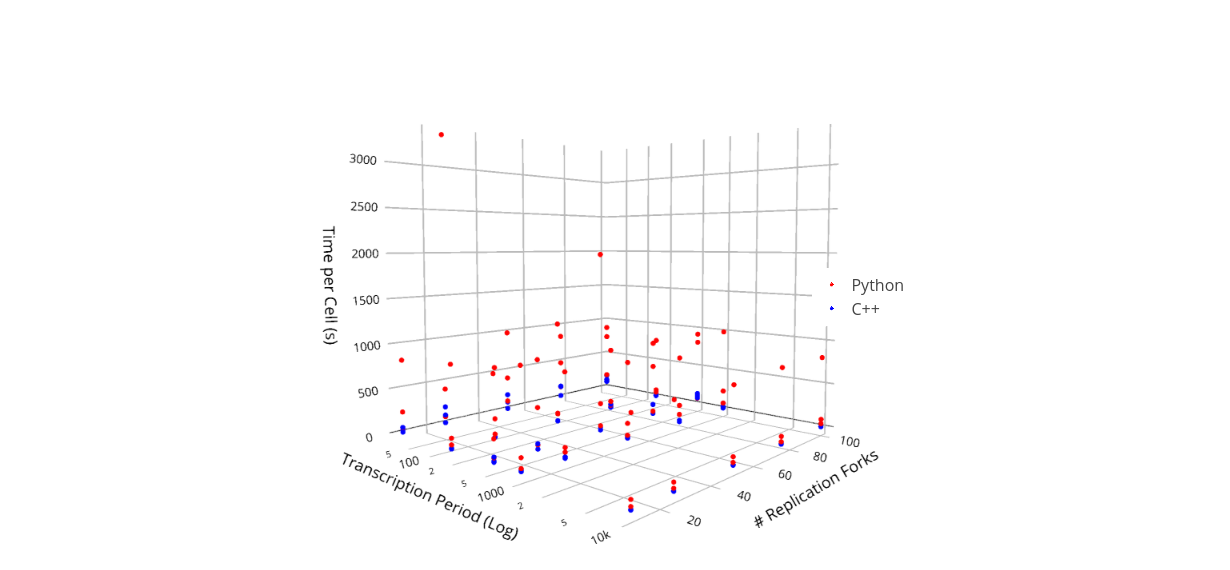
\includegraphics[trim = 105mm 10mm 55mm 40mm, clip=true]{time_plot.png}}
    }
    \label{fig:time_comparison}
\end{figure}
{\bf Fig.~2: Performance comparison between C++ and Python implementations.} In this assay, we compared the Python version of the ReDyMo simulator (red dots) with its C++ port (blue dots). We tested both simulations with different values for transcription frequency and number of replication forks. For each pair of these parameters, we carried out batches of 1, 10, and 100 simulations, one batch at a time. In the case of the 100-simulations batch, up to 40 simulations were executed at the same time. On average, C++ simulations required only 8 \% of the Python computational time.
}
\end{block}                     
                     
\begin{block}{Results and Single-Factor Models}
\parbox[t][]{0.95\textwidth}
{
\begin{figure}
    %\centerline{\scalebox{1.8}{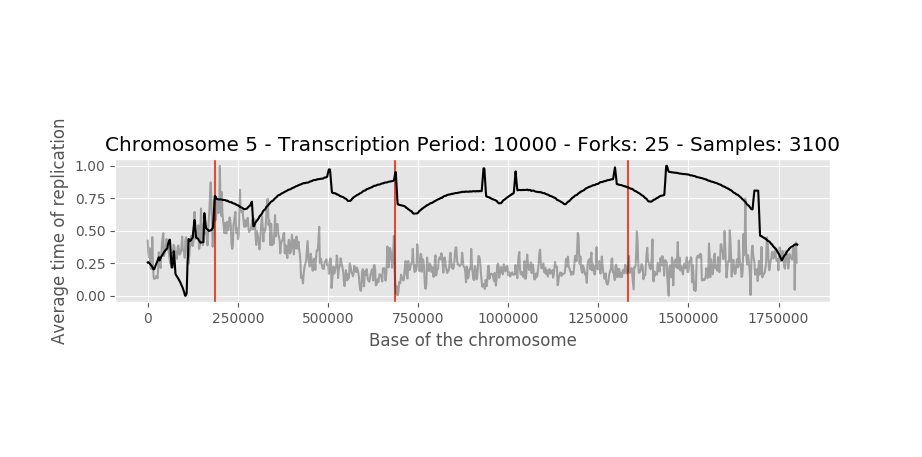
\includegraphics[trim = 10mm 20mm 10mm 30mm, clip=true]{best_ro_3k.png}}}
    \centerline{\scalebox{1.5}{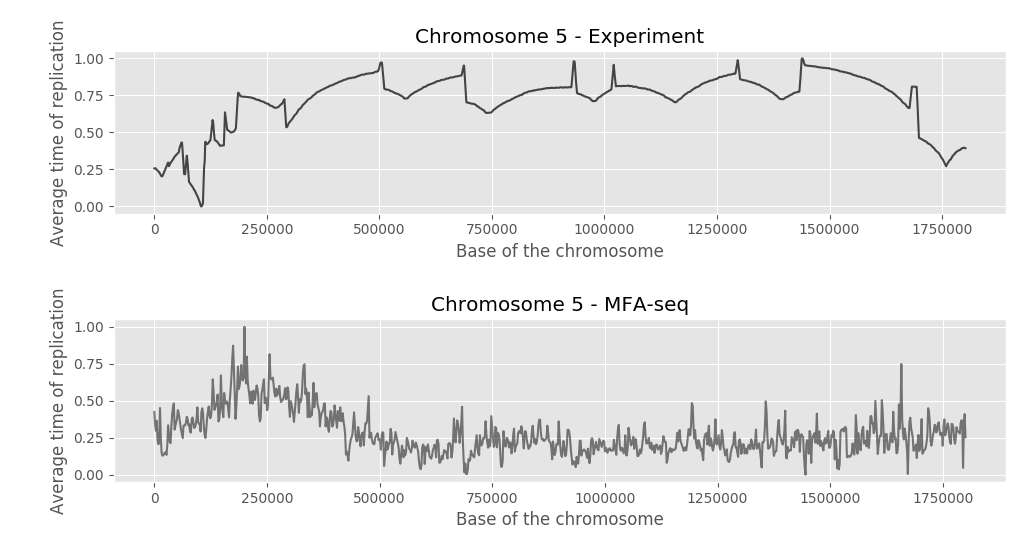
\includegraphics[trim = 10mm 0mm 0mm 0mm, clip=true]{mfa_exp.png}}}
    \label{fig:best_ro}
\end{figure}
{\bf Fig.~3: Simulations with uniform probability of origin firing along the genome.}  In this experiment, we carried out 3,000 independent simulations, each one with transcription period equal to 10,000 simulation iterations and 25 replication forks. Then we split each chromosome into 1,000 equally-sized bins. For each simulation and for each bin, we computed the mean iteration that each base was replicated. Finally, for each 
       }
\end{block}  
\vskip1ex


\begin{block}{Conclusions}
\parbox[t][]{0.95\textwidth}
{
\begin{itemize}
\item We implemented and tested a C++ port of ReDyMo, which is much more efficient than the Python-based version\\
\vskip1ex
\bigskip
\item We used this new version to show preliminary results that suggest an influence of transcription activity (i.e., its conflicts with replication forks) on the origin firing positioning\\
\bigskip
\item Next step is the implementation of the outer layer of the multiscale model within the FLAME framework.
\vskip1ex
\end{itemize}
}
\end{block}
\vskip1ex
      
      \vfill  % last vfill is important to avoid page duplication!

} % end \parbox

\end{minipage}
\end{beamercolorbox}
\end{column}
% ---------------------------------------------------------%
% end the column
\end{columns}

\vskip1ex

\end{frame}

\end{document}

% End of file.
%
